\documentclass[letterpaper,12pt]{article}


\listfiles

%\usepackage{setspace}
%\doublespacing
\usepackage{pdfcomment}
%usepackage{hyperref}
\hypersetup{hidelinks}

%%  Accepte les caractères accentués dans le document (UTF-8).
\usepackage[utf8]{inputenc}
%\usepackage[french]{babel}
\usepackage[T1]{fontenc}

\usepackage[bb=boondox]{mathalfa}




%change les references aux equations
%\let\oldref\ref
%\renewcommand{\ref}[1]{\in@{eq:}{#1} \ifin@ (\oldref{#1}) \else \oldref{#1} \fi}

%commentaires
\usepackage{verbatim}

%double espacement
\usepackage{setspace}
% \doublespacing

%notes sur le pdf


%------------------------------
%packages pour tableaux
\usepackage[table,xcdraw]{xcolor}
\usepackage{rotating}

%-----------------------------

%packages pour figures
%\usepackage{fancybox}
\usepackage{epsfig}
\usepackage{graphicx}


%------------------------------------------------
%Bibliographie

%ancienne
%\usepackage[round]{natbib}
%\usepackage{numcompress}
%\bibliographystyle{model4-names}

% Natbib setup for author-year style
\usepackage{natbib}
\bibpunct[, ]{(}{)}{,}{a}{}{,}%
\def\bibfont{\small}%
\def\bibsep{\smallskipamount}%
\def\bibhang{24pt}%
\def\newblock{\ }%
\def\BIBand{and}%
\bibliographystyle{informs2014trsc}

%\usepackage[strings]{underscore}
%\bibliographystyle{plainnat}
%------------------------------------------------

%-----------------------------------------
%TIKZ
\usepackage{tikz}
\usetikzlibrary{arrows,shapes,positioning,shadows,trees}
\usetikzlibrary{patterns}
\usetikzlibrary{calc, graphs}


\tikzset{hide on/.code={\only<#1>{\color{fg!20}}}}
\tikzset{
	invisible/.style={opacity=0},
	visible on/.style={alt=#1{}{invisible}},
	alt/.code args={<#1>#2#3}{%
		\alt<#1>{\pgfkeysalso{#2}}{\pgfkeysalso{#3}} % \pgfkeysalso doesn't change the path
	},
} 
\tikzset{
	depnode/.style={circle, minimum size=0.3cm, draw, thin},
	arrnode/.style={circle, minimum size=0.3cm, draw, thin, fill=black},
	waitnode/.style={circle, minimum size=0.3cm, draw, thin, pattern = north east lines},
	sourcesinknode/.style={circle, draw, minimum size=0.3cm, line width=0.1cm},
	wait/.style={->, >=triangle 45, thin},
	nullarc/.style={->, >=open triangle 45, thin},
	flight/.style={->, >=stealth, thin},
	deadhead/.style={->, >=stealth, thin, bend left=10, dashed},
	connect/.style={->, >=open diamond, thin},
	rest/.style={->, >=diamond, thin},
	begend/.style={->, >=stealth, thick, dotted}
}
%-------------------------------------------


%packages de math
\usepackage{amssymb}
\usepackage{amsmath}

\usepackage{caption}

%packages divers
\usepackage{enumerate}
\usepackage[top=1in, bottom=1in, left=1in, right=1in]{geometry}

%packagespour tableaux
\usepackage{multirow}
%\renewcommand{\arraystretch}{0.6}

%packages et commande pour décrire les algorithmes
%\usepackage{algorithm}
%\usepackage{algorithmicx}
%\usepackage{algpseudocode}

%packages pour bibliographie

%% Vancouver numbered
%\usepackage{numcompress}\bibliographystyle{model3-num-names}
%\usepackage{natbib}
%\usepackage{bibentry}

%couleur
\usepackage{color}



%commandes personnalisées

%mettre parentheses automatiquement aux references
\let\oldref\ref
\makeatletter
\newcommand\myref[1]{\oldref{#1}}
\makeatother
%les accolades supplémentaires sont pour que tout soit inclus dans les commandes comme les exposants (on peut faire $x^\ref{...}$)
\renewcommand{\ref}[1]{{\myref{#1}}}
\renewcommand{\eqref}[1]{{(\myref{#1})}}

\renewcommand*{\thesubsection}{Question \arabic{section}.\arabic{subsection}}

\newcommand{\red}[1]{{\color{red}[#1]}}
\newcommand{\new}[1]{{\bfseries#1}}
\usepackage[breakable]{tcolorbox}
\newcommand{\nouveau}[2][]{
	\begin{center}
		\begin{tcolorbox}[left=0pt, right=0pt, boxsep=5pt, width=1.03\textwidth, colframe=red!75!black,title={\textbf{\Large Nouveau! #1}},coltitle=black, colbacktitle=white, colback=white, breakable]
			#2
			
		\end{tcolorbox} 
	\end{center}
}

\newcommand{\note}[1]{\red{#1}}



%\renewcommand{\baselinestretch}{1.5} 

\title{ Optimisation de la production d'une mine à ciel ouvert }
\author{\textsc{\large{Frédéric Quesnel}} \\ MTH6601}

%\date{\today}

%\baselineskip=15pt

\begin{document}
	
	\maketitle
	
	\setcounter{section}{-1}
	\section{Avant de commencer...}
	Ce TP concerne l'optimisation des opérations d'une mine à ciel ouvert. Il est basé sur un vrai projet de recherche mené par un professeur de Polytechnique. Dans ce TP, vous étudirez un modèle simplifié de mine à ciel ouvert à l'aide d'un simulateur. Une présentation décrivant le fonctionnement de la mine et du simulateur se trouve sur Moodle. Il est fortement recommandé de relire ce document avant de commencer. Pour toute question concernant le simulateur ou cet énoncé, ou encore pour signaler un bogue du simulateur, n'hésitez pas à contacter à Frédéric Quesnel. 
	
	
	Il est encouragé d'inclure des tableaux ou des graphiques pertinents à vos réponses. Toutefois, le coeur de l'évaluation portera sur votre analyse et vos conclusions. 
	
	
	%---------------------------------------------------------------------------------------------------------
	\section{Prédiction des temps de parcours}
	
	Le temps de parcours d’un camion sur un chemin varie de manière stochastique, et peut être influencé par divers facteurs tels que l’état de la route ou la météo. Il est important d'être en mesure d'estimer correctement ces temps de parcours afin de bien planifier les opérations. Dans cette section, vous étudierez trois formules qui peuvent être utilisées pour estimer les temps de parcours. 
	
	Lorsqu'un camion débute un trajet, la formule de prédiction estime son temps de parcours. Il s'agit du \textit{temps de parcours prédit}. Lorsque le camion arrive à sa destination, son \textit{temps de parcours observé} est enregistré. Dams le simulateur, le graphe \textit{Temps de parcours observés et prédits} affiche les temps observés et prédits des camions sur deux chemins spécifiques (la légende indique de quels chemins il s'agit).
	
	
	Soient $t_{ij}^k$ et $t^{*k}_{ij}$ les temps prédits et observés pour le segment (chemin) $(i,j)$ à l'instant $k$. $t_{ij}^{k-1}$ et $t^{*k-1}_{ij}$ dénotent les temps prédits et observés du dernier camion sur le segment $(i, j)$ à être arrivé avant l'instant $k$. Soit $A$ l'ensemble des segments. Le logiciel de simulation propose les trois formules suivantes pour estimer le temps de parcours d’un camion sur le segment $(i,j)$ : 
	
	
	\begin{itemize}
		
		\item Moyenne des observations précédentes (sur le même segment)
		
		\begin{equation}
		t_{ij}^k = \frac{1}{n} \sum\limits_{k=1}^n t_{ij}^{*k-1}
		\end{equation}
		
		\item Combinaison convexe
		
		\begin{equation}
		t_{ij}^k = \lambda t^{*k-1}_{ij} + (1-\lambda) t_{ij}^{k-1} \qquad \lambda \in [0, 1]
		\end{equation}
		
		\item Erreur précédente
		
		\begin{equation}
		t_{ij}^k = \lambda t^{*k-1}_{ij} + (1-\lambda) t_{ij}^{k-1} \left( 1- \frac{\sum\limits_{(l,m) \in A} t_{lm}^{k-1} - t_{lm}^{*k-1}}{\sum\limits_{(l,m) \in A} t_{lm}^{*k-1}}\right)
		\end{equation}
		
		
	\end{itemize}
	
	L'interface permet de modifier les valeurs de $n$ et $\lambda$ pour chaque formule.
	
	\subsection*{Protocole expérimental pour cette section : }
	
	\begin{itemize}
		\item Mine : 4 pelles
		\item Nombre de camions : 20
		\item Temps de simulation : 24h
		\item Fonction de score : « aléatoire » (option par défaut)
	\end{itemize}
	
	Étapes de simulation : 
	\begin{enumerate}
		\item Lancer la simulation à l’aide du bouton play (pour voir l’animation).
		\item Attendre au moins 3h de simulation (pour que les formules de prédictions se stabilisent).
		\item Varier la température (de neige à soleil, ou l’inverse).
		\item Attendre que la formule de prédiction se stabilise de nouveau, ou la fin de la simulation.
	\end{enumerate}
	
	
	
	\subsection{}
	
	Les trois fonctions ci-dessus adaptent leurs prédictions en se basant sur les observations
	précédentes. Donnez deux comportements désirables d'une formule de prédiction.
	
	\begin{comment}
	\textbf{Réponse : }
	
	\begin{itemize}
		\item Bonne valeur de prédiction en régime stable.
		\item S'adapte rapidement aux changements de conditions.
		\item Peu sensible aux données aberrantes (ex. si un camion tombe en panne).
	\end{itemize} 
	\end{comment}
	%L’objectif est de trouver une formule de prédiction qui réagit rapidement lors de changements drastiques des conditions de conduites sur l’ensemble de la mine.
	
	
	
	
	
	
	\subsection{}
	Observez le comportement de la formule « Moyenne des observations précédentes » avec différentes valeurs de $n$. Quels sont les avantages et les inconvénients à utiliser une plus grande valeur de $n$. 
	
	\subsection{}
	En utilisant la formule « combinaison convexe », on observe que plus la valeur de $\lambda$ est grande, plus la formule s’adapte rapidement aux changements de température. Doit-on conclure qu’il vaut mieux utiliser $\lambda=1$? Pourquoi?
	
	\subsection{}
	La formule « Erreur précédente » est celle qui s’adapte le plus rapidement aux changements de conditions météorologiques. 
	\begin{itemize}
		\item Comment expliquez-vous ce phénomène? 
		\item Si d’autres facteurs que la météo affectaient le temps de déplacement (par exemple, la détérioration soudaine d'une route), la formule "erreur précédente" serait-elle encore valide? Justifiez.
	\end{itemize}

	\subsection{}
	En général, les formules de prédiction semblent plus précises sur le chemin \textit{concentrateur:pelle1} que sur le chemin \textit{sterile:pelle3}. Comment expliquez-vous cela?
	
	\subsection{}
	
	Pour cette question, supposez que les temps de transport et de remplissage sont déterministes. Supposons que $n$ camions sont en route pour la pelle et que $m$ camions sont déjà en attente à celle-ci. Soit $t_i$ le temps que prend le camion $i$ pour arriver à la pelle, en secondes, et supposons que les camions sont ordonnés par ordre de temps d'arrivée à la pelle ($t_1 \leq t_2 \leq ...\leq t_{n-1} \leq t_n$). Un camion est en cours de remplissage, et ce remplissage sera complété dans $t^r$ secondes. Le temps de remplissage d'un camion est de $T^R$ secondes. Cette situation est illustrée sur la figure \ref{fig:file}.
	
	\begin{figure}
		\center
		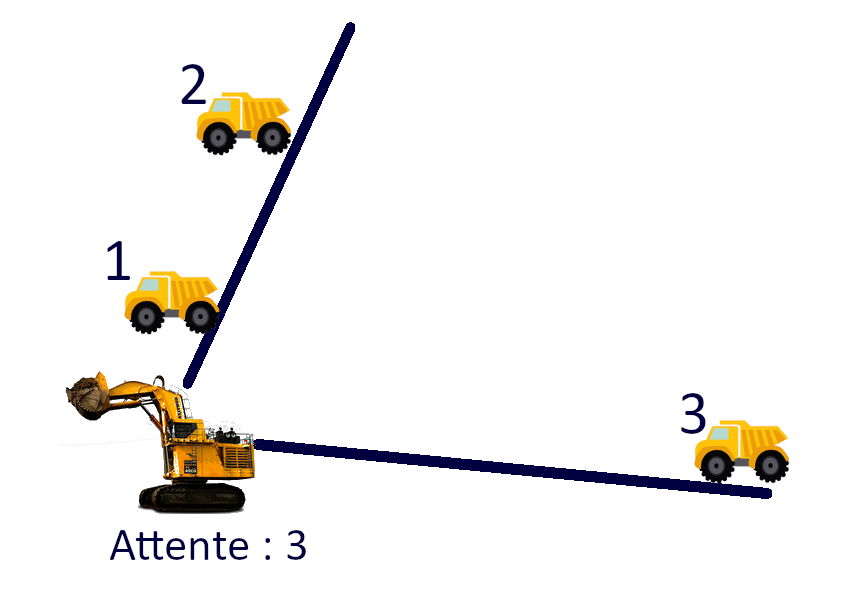
\includegraphics[width=0.4\linewidth]{File.png}
		\caption{\label{fig:file}}
	\end{figure}
	
	Donnez une formule permettant de calculer dans combien de temps débutera le remplissage du camion $n$.
	
	\textbf{Indice :} Vous pouvez utiliser une équation de récurrence.
	
	%---------------------------------------------------------------------------------------------------------
	\section{Affectation des camions un par un}
	\label{sec:score}
	Lorsqu'un camion arrive au concentrateur ou à la pile de stérile, il se décharge instantanément et devient disponible. On doit alors lui assigner une nouvelle destination. Le but de cette section est de déterminer une règle qui assigne au camion sa prochaine destination (pelle). L'assignation se fait de la manière suivante : un score est calculé pour l'assignation du camion à chaque pelle. La pelle avec le \textbf{plus petit} score est choisie (en cas d'égalité, la pelle avec le plus petit numéro est choisie).
	
	\subsection*{Protocole expérimental : }
	
	\begin{itemize}
		\item Mine : 10 pelles
		\item Nombre de camions : 20
		\item Temps de simulation : 24h
		\item Fonction de score : votre fonction de score.
	\end{itemize}
	
	Étapes de simulation : 
	\begin{enumerate}
		\item Lancer la simulation (à l'aide du bouton \textit{play}, ou \textit{compléter auto)}.
		\item   Enregistrer les résultats.
	\end{enumerate}
	
	\textbf{Astuce : }N'hésitez pas à utiliser la mine à 4 pelles, ou un nombre moins élevé de camions pour déboguer vos fonctions de score!
	
	\subsection{} 
	
	Vous désirez optimiser la production totale (minerai + stérile), sans tenir compte du plan de travail des pelles. 
	
	Par défaut, l'assignation se fait à partir de la fonction écrite dans le champ \textit{fonction de score} de l'interface graphique. Vous devez élaborer une fonction de score à l'aide des variables fournies dans la section \ref{sec:vars}, ainsi que des opérations élémentaires (+, -, *, /, \%). Les exposants peuvent également être utilisés à l'aide de la fonction Java {\verb Math.pow([base], [exopsant])}. Par exemple, entrer la formule "n1" envoie toujours un camion disponible à la pelle ayant le moins de camions en attente.
	
	
	
	Expliquez votre choix de fonction de score. Observez-vous une hausse de productivité (par rapport à une assignation aléatoire)? Si oui, de combien? 
	
	
	
	\begin{comment}
	\subsection*{Question 2.2} 
	Vous pouvez créer des règles de décision plus complexes en modifiant les fonctions identifiées ({\verb computeDecisionScore} et {\verb computeCustomDecisionScore}) dans le fichier 
	
	\noindent{\verb CustomDecisionMaker.java}. La fonction {\verb computeCustomDecisionScore} vous donne accès à l'ensemble des camions, aux pelles, et à la mine en général (la documentation de ces classes est fournie avec le code). Vous pouvez également utiliser les variables définies au début du fichier. 
	
	Si possible, créez une règle de décision permettant d'améliorer la productivité. Donnez une brève description de votre algorithme.
	\end{comment}
	
	\subsection{}
	
	
	On souhaite maintenant optimiser la production tout en respectant les contraintes suivantes : 
	
	\begin{itemize}
		\item \textbf{Maximiser : }  Production au concentrateur + 0.2 $\times$ Production au stérile
		\item Au maximum 25\% de la production doit être du stérile.
		\item Le concentrateur doit avoir au plus 1.9\% de soufre, et entre 26\% et 27\% de fer.
	\end{itemize}
	
	Vous devez créer une fonction de score permettant d'arriver à cet objectif en modifiant les fonctions (\verb computeDecisionScore $\;$et \verb computeCustomDecisionScore) dans le fichier \verb CustomDecisionMaker.java. La fonction \verb!computeCustomDecisionScore! vous donne accès à l'ensemble des camions, aux pelles, et à la mine en général (la documentation de ces classes est fournie avec le code). Vous pouvez également utiliser les variables définies au début du fichier. 
	
	\begin{itemize}
		\item Décrivez brièvement votre fonction et expliquez le raisonnement derrière celle-ci.
		\item Donnez une mesure de performances (moyenne sur plusieurs simulations) de votre fonction (quantité totale produite, respect des contraintes de production...)
	\end{itemize}
	
	
	
	%---------------------------------------------------------------------------------------------------------
	\section{Problème d'affectation}
	
	On désire maintenant affecter les camions en tenant compte des camions qui seront prochainement disponibles. Pour ce faire, on résout un problème d'affectation tel que décrit dans la présentation sur Moodle. Vous pouvez activer le problème d'affectation en écrivant "optimise" dans le champ de la fonction de score. Vous pouvez également affecter les camions un à un, mais avec la même fonction de score que pour le problème d'affectation, en écrivant "optimal\_assign" dans le champ de la fonction de score.
	
	On souhaite également prendre en compte le \textit{plan d'opération} de la mine. Un plan d'opération indique le nombre cible de camions par heure qui doivent aller à chaque pelle afin de respecter les besoins de production. La cible de chaque pelle est indiquée en vert à côté de celle-ci.
	
	
	\subsection*{Protocole expérimental : }
	
	\begin{itemize}
		\item Mine : 10 pelles
		\item Nombre de camions : 20
		\item Temps de simulation : 24h
		\item Fonction de score : optimise.
	\end{itemize}
	
	
	
	\subsection{}
	
	Donnez un exemple hypothétique pour lequel il est avantageux d'utiliser un problème d'affectation par rapport à assigner les camions un par un.
	
	\subsubsection{} 
	
	Effectuez des simulations pour comparer l'affectation des camions "un par un" à l'affectation des camions avec un problème d'affectation. Comparez également avec vos résultats de la question 2.2.
	
	Quels sont les effets sur :
	
	\begin{itemize}
		\item la production totale.
		\item le respect du plan.
		\item la composition du mélange.
	\end{itemize}
	
	\subsubsection*{Question 3.3}
	Utiliser directement la formule $c_{ij} = \left(E(AC)-AC\right)^2 + \left(E(AP)-AP\right)^2$ (voir présentation sur Moodle) dans le problème d'affectation peut parfois poser problème. Expliquez pourquoi. Proposez ensuite une solution à ce problème.
	
	
	
	
	%---------------------------------------------------------------------------------------------------------
	\section{Modification du plan d'opération}
	
	Le plan d'opérations peut être modifié dans le but d'atteindre divers objectifs de production. Pour modifier la cible d'une pelle, effectuez un clic droit sur la pelle, cliquez sur "Modifier le plan", et entrez la valeur désirée. La capacité maximum d'une pelle est de \textbf{6 camions} par heures. Pour remettre les valeurs par défaut, chargez la mine de nouveau.
	
	
	
	
	\subsection*{Protocole expérimental : }
	
	\begin{itemize}
		\item Mine : 10 pelles
		\item Nombre de camions : 20
		\item Temps de simulation : 24h
		\item Fonction de score : optimise ou optimal\_assign.
	\end{itemize}
	
	\subsection{}
	Supposez que le plan actuel est suivi à la lettre. Estimez quelle devrait être, sur une période de 24h : 
	
	\begin{itemize}
		\item La quantité de minerai livrée au concentrateur.
		\item La quantité de stérile livrée à la pile de stérile.
		\item Le pourcentage de fer et de soufre au concentrateur.
	\end{itemize}
	
	Comparez ces chiffres avec les résultats d'une simulation.
	
	\subsection{}
	En supposant que tout plan peut être suivi à la lettre, écrivez un modèle d'optimisation linéaire qui détermine le meilleur plan d'opérations en régime continu. 
	
	\begin{itemize}
		\item \textbf{Maximiser : }  Production au concentrateur + 0.2 $\times$ Production au stérile
		\item Au maximum 25\% de la production doit être du stérile.
		\item Le concentrateur doit avoir au plus 1.9\% de soufre, et entre 26\% et 27\% de fer.
	\end{itemize}
	
	À l'aide d'un logiciel d'optimisation (le solveur d'Excel, par exemple), résolvez ce problème et donnez sa solution. Répondez ensuite à la première partie de la question 4.1 en utilisant ce plan (sans faire de simulation).
	
	\subsection{}
	
	Simulez le plan trouvé en 4.2. Comparez les résultats de la simulation avec les prédictions du logiciel d'optimisation. Selon vous, qu'est-ce qui explique ces différences? Autrement dit, quels sont les éléments que le modèle d'optimisation linéaire ne considère pas.
	
	\subsection{}
	
	Proposez un plan d'opération qui permet de respecter toutes les contraintes (dans une simulation). Simulez ce plan et donnez-en les caractéristiques de production.
	
	\subsection{}
	Les modèles linéaires ont tendance à produire des solutions extrêmes. Expliquez en quoi cela pourrait être un problème avec le modèle développé en 4.2.
	
	
	
	
	
	
	\section{Optimisation des coûts de production}
	%---------------------------------------------------------------------------------------------------------
	
	Si le coût pour une minute d’attente d’une pelle est 10\$, et que l’attente d’un camion coûte 3\$/minute, estimez le nombre optimal de camions (nombre de camions qui minimise le coût total d'attente)? Utilisez le plan par défaut.
	
	
	\section*{Question bonus?}
	Il pourrait être utile de développer un outil qui indique au planificateur si son plan est réaliste.
	
	Donnez un problème d'optimisation qui calcule le plus petit nombre de camions nécessaires pour respecter un plan donné. (Indice : il s'agit d'un problème de transport qui minimise le temps \underline{total} d'opération des camions en régime continu).
	
	
	\section{Liste des variables}
	\label{sec:vars}
	
	
	\begin{itemize}
		\setlength\itemsep{0.01em}
		\item $x1$ : Vitesse moyenne d'un camion.
		\item $x2$ : Vaut 1 si la pelle est actives, 0 sinon.
		\item $x3$ : Nombre réel aléatoire entre 0 et 1.
		\item $x4$ : Infini ($(2-2^{-52})*2^{1023}$)
		\item $t1$ : Temps moyen de remplissage d'un camion.
		\item $t2$ : Temps de parcours espéré jusqu'à la pelle.  
		\item $d1$ : Distance entre le camion et la pelle.
		\item $n1$ : Nombre de camions en attente (sans compter le camion en remplissage).
		\item $n2$ : Nombre de camions à la pelle (en comptant le camion en remplissage).
		\item $n3$ : Nombre de camions en route pour la pelle.
		\item $t3$ : Temps espéré avant que la pelle n'ait terminé le remplissage des camions actuellement en attente.
		\item $t4$ : Temps espéré avant le début du remplissage du camion.
		\item $t5$ : Temps d'attente espéré du camion (0 si la pelle est inactive quand le camion arrive).
		\item $t6$ : Temps d'attente espéré de la pelle (peut être négatif si le camion arrive avant que la pelle ne soit en attente).
	\end{itemize}
	
	
	
\end{document}

